\section{Benchmarks}

A set of common benchmarks are used to evaluate the reliability related properties of the different frameworks. The benchmarks used are polybench and axbench. 

Polybench is a set of benchmarks that test common workloads (or kernels) running on CPUs. There is also a polybench benchmark suite for GPU applications, but this project focuses on CPU applications. 

Out of the box, polybench runs the kernels, and provides a result in the form of amount of seconds each benchmark was run. The TAFFO project has taken this benchmark and modified it to run all the kernels both for an unmodified version of clang as well as their own reduced precision compiler, and then gives time spent on both results, as well as the error of the reduced precision compiler. 

Numerical accuracy (loss) alone does not say anything about fault tolerance, therefore this necessitates the addition of more metrics.

One measure that may be interesting to record is the amount of cycles a benchmark is completed in. in addition to potentially being a measure that is easier to compare between different machines that have different clock speeds, it would be interesting to see how faults may affect the amount of cycles that the CPU has to perform.

other measures:

types of faults! as described in gem-5 approxylizer?
Should collect different types of faults for different tools: to what degree to the faults become errors?
    should look at developmental faults in addition to operational faults. Metric for this? Need to look at the faults that crop up in relation to each other rather than an absolute measure

gem5-approxilyzer uses the following error model:
"The error model we use is single-bit transient errors in
architectural registers. We study errors in bits of both source
and destination registers of instructions." (cited) 

It is interesting to identify faults that in approximate computing systems result in unacceptable Silent Data Corruptions (SDCs) vs acceptable SDCs in non-approximate computing systems- or potentially the other way around!
The approxilyzer has obvious limits, one being the simple error model. The error model assumes single bit-errors, but does not look at combinations of flipped bits (as far as I can understand now...)

What else could be interesting to monitor:

- cycles
- faults
    - SDC (acceptable, non-acceptable)
    - managed
    - failures
- time?
- loss in accuracy
- reliability:
    - ratio of change in non-acceptable vs acceptable SDC
    - ratio of change in failures
    - cycle cost of mitigating failures


Want to measure developmental faults as well. 
    - mutation testing
    - statistics of the code base:
        - reported bugs
        in relation with:
        - development speed/efficiency (?) 
            - commits / week
            - LoC / week
            - features / month

    Not measuring statistics! 
    Injecting different types of developmental faults, and evaluating their effects.

Looking at floatsmith: tool that makes it easier to run benchmarks. Given up on Taffo! Difficult to set up! Only supports certain versions of llvm. difficult to maintain LLVM-compatible tools when toolchain changes a lot around it. Also difficult to set up, requires a lot of work to get working, have to build llvm from source and then build taffo, a lot of errors with dependencies. (create tests for configuration of system??)


First injecting developmental faults.  
Both floatsmith and TAFFO are not neccessarily plug and play, which is a shame. Why not pre-built solution? Why does not TAFFO have an option that performs builds from the ground up? if it is dependent on llvm-15, why no build status...


Usage of the tools is not easy, documentation (at least for floatsmith) is not bountiful. Though this is not a study on how easy the tools are to use!!

Floatsmith requires the code's build method to be able to build and run the code to find speedups. In addition to this floatsmith may require some prerequisite knowledge of the internals of floatsmith. Attempting to run the pre-built floatsmith image on a code project that builds using multiple different build scripts as well as specialized run commands, it is not able to correctly build and run the code. Floatsmith need reference input and output to work, to enable finding the accuracy of the different mixed precision version. 

Ref the last paper leonardo recommended:
Errors depend on the observer. A perfect observer with complete overview of factors both internal and external to the program will be able to distinguish faults clearly, as well as distinguishing a timing error from an omission error.
Human users are not perfect observers. based on an input, it is not always possible to decide whether a result is an error or a correct value, especially given that there is an output at all. 
Timing errors, over a threshold time, are difficult/impossible to distinguish from omitted output.  (what kind of faults can cause this type of error? buffer overflow causing crash?)

injecting faulty data is not fault injection, but injection of \textit{the result of} a fault, i.e. an error.

Error injection is proven to be valuable for robustness testing. (on fault representativeness says that representativeness is not an issue in robustness testing because the goal is to find weaknesses?? If faults are not representative then you still do not catch a large group of faults??)

Need fault statistics such as with G-SWFIT? Are there statistics for HPC applications? use generic fault distribution. 

Want to focus on syntactically correct faults using generic fault distribution *onFaultRepresentativeness

Faults most relevant to reduced precision computation, specifically float to fixed or float to (smaller) float:
MLPA = missing small and localized part of the algorithm
WVAV = wrong value assigned to variable

These could be direct errors that could come from editing source code to reduce precision, but other faults that could be investigated either as (følgefeil) or some other issues. 

MFC = missing function call
MVIV = Missing Variable Initialization using a value
MVAE = missing variable assignment using an expression
WPFV = wrong variable used in parameter of function call
WAEP = wrong arithmetic expression in parameter of function call


The paper on fault representativeness focuses on applications outside the HPC domain. This is not explicitly stated to be the focus of this thesis, but it is in HPC and scientific computation domain that approximate computing can produce the largest payoffs. Approximate computing in other fields, such as web servers, can be performed through the use of e.g. cached responses (memoization) for computation-heavy requests, resulting in a response that may be outdated, and therefore approximately correct (dependent on the domain: some services have higher requirements for QoS than others). 

Since techniques such as memoization, loop perforation and ... are not readily available as tools proven to work, evaluating their effect on reliability may only be done in theory. Essentially, tools such as Green are useless since the implementation does not exist. The tool itself is not reproducible from the paper. Silly little thing. 


Assuming that the values in the file vra.txt (where the benchmark times are stored for all the polybench results) not all situations where variables are converted from floating point variables to fixed point variables result in a speedup, there are many results that result in a slower average execution time. (could this be because of my computer? have to run some checks on the other computers to see whether the results are different)


The biggest speedup comes from the seidel-2d benchmark, will look at that.

It is interesting to verify whether the speedup gained from using fixed point variables comes at the cost of reliability. This is perhaps the most interesting thing to verify, or the result (if I can get it verified) that makes the project worthwhile.


Injected errors: I think it is neccessary to look at domain-specific errors: e.g. inject errors inside TAFFO annotations, how can this affect the program? 
Still no good grouping of errors. I am not sure what kinds of errors I should inject! Need to start simple:
I will try to inject simple faults to crash the program. Will run it with cmake, ignoring errors, and comparing between approximated code and non-approximated code. 
Then I can think about other facets. Start simple

Where do I go from there? Detectability? 
More code = more potential for error?
Static analysis of annotations?
create simple llvm pass that performs loop perforation? only if annotated  
    Other approximate computing techniques:
    memoization? Can this be done dynamically?




Started performing fault injection.

First, doing fault injection on seidel-2d benchmark in polybench suite. This is because TAFFO has pre-made build and execute scripts that may help with simplifying usage. 
There is a "validate" script that outputs the average results of the execution, giving absolute (average) error and error percentage, as well as potential speedup. Some of the benchmarks don't even achieve speedups when using fixed point implementation instead of floating point representation.
The validate script was not very clearly written, so I had to investigate what the variables actually meant and what the output actually meant. After doing this I could start the fault injection.

First I injected some simple faults (what are they called again...) in the logic operators in loops, to see whether the program still ran, and whether accuracy dropped differently between the two variables.
\begin{figure}
    \centering
    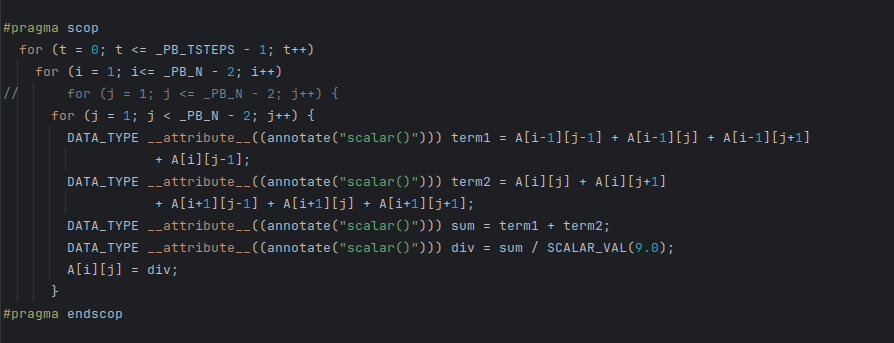
\includegraphics[width=0.5\linewidth]{Images/injected_basic_error.png}
    \caption{injected error}
    \label{fig:enter-label}
\end{figure}

slightly higher error in the fault injected version. This means that the fault caused a bigger discrepancy in the fixed point implementation than the floating point implementation:

\begin{verbatim}
[01:07 PM]-[lars@lars-Latitude-7310]-[~/.../test/fault-injected-polybench-cpu]- |improve_readability U:1 ?:15 ✗|
$ ./run_faulty_seidel_benchmark.sh 
[ ok ] ./stencils/seidel-2d/faulty-seidel-2d.c
[ ok ] ./stencils/seidel-2d/faulty-seidel-2d.c
          avg_absolute_error          avg_percentage_error                 fixed_point_time_average fixed_point_value_invalid_count floating_point_time_average floating_point_value_invalid_count speedup                       
seidel-2d  0.000102257390319354703125  0.0001017454833562187286071162135 %  0.077007 seconds         0                               0.141137 seconds            0                                  1.832781435453919773527081954

[01:07 PM]-[lars@lars-Latitude-7310]-[~/.../test/fault-injected-polybench-cpu]- |improve_readability U:1 ?:15 ✗|
$ ./run_seidel_benchmark.sh 
[ ok ] ./stencils/seidel-2d/seidel-2d.c
[ ok ] ./stencils/seidel-2d/seidel-2d.c
          avg_absolute_error          avg_percentage_error                 fixed_point_time_average fixed_point_value_invalid_count floating_point_time_average floating_point_value_invalid_count speedup                       
seidel-2d  0.000102525901793475199375  0.0001020126506449179568796360769 %  0.077005 seconds         0                               0.144294 seconds            0                                  1.873826374910720083111486267
\end{verbatim}


further modifications below:
\begin{verbatim}
    #pragma scop
//  for (t = 0; t <= _PB_TSTEPS - 1; t++)
  for (t = 0; t < _PB_TSTEPS - 1; t++)
//    for (i = 1; i<= _PB_N - 2; i++)
    for (i = 1; i < _PB_N - 2; i++)
//      for (j = 1; j <= _PB_N - 2; j++) {
      for (j = 1; j < _PB_N - 2; j++) {
        DATA_TYPE __attribute__((annotate("scalar()"))) term1 = A[i-1][j-1] + A[i-1][j] + A[i-1][j+1]
                   + A[i][j-1];
        DATA_TYPE __attribute__((annotate("scalar()"))) term2 = A[i][j] + A[i][j+1]
                   + A[i+1][j-1] + A[i+1][j] + A[i+1][j+1];
        DATA_TYPE __attribute__((annotate("scalar()"))) sum = term1 + term2;
        DATA_TYPE __attribute__((annotate("scalar()"))) div = sum / SCALAR_VAL(9.0);
        A[i][j] = div;
      }
#pragma endscop
\end{verbatim}

resulted in these results:
\begin{verbatim}
    $ ./run_faulty_seidel_benchmark.sh 
[ ok ] ./stencils/seidel-2d/faulty-seidel-2d.c
[ ok ] ./stencils/seidel-2d/faulty-seidel-2d.c
          avg_absolute_error         avg_percentage_error                 fixed_point_invalid_result_count fixed_point_time_average floating_point_invalid_result_count floating_point_time_average speedup                       
seidel-2d  0.00010099707543756559375  0.0001004914776904355906214804212 %  0                                0.105733 seconds         0                                   0.206827 seconds            1.956125334569150596313355338


\end{verbatim}


testing simple fault injection in loop:
code: (commented out code is the correct code, code just below is fault injected code)
\begin{verbatim}
  for (t = 0; t <= _PB_TSTEPS - 1; t++)
    for (i = 1; i<= _PB_N - 2; i++)
      for (j = 1; j <= _PB_N - 2; j++) {
//        DATA_TYPE __attribute__((annotate("scalar()"))) term1 = A[i-1][j-1] + A[i-1][j] + A[i-1][j+1]
//                   + A[i][j-1];
        DATA_TYPE __attribute__((annotate("scalar()"))) term1 = A[i-1][j] + A[i-1][j] + A[i-1][j+1]
                   + A[i][j-1];
        DATA_TYPE __attribute__((annotate("scalar()"))) term2 = A[i][j] + A[i][j+1]
                   + A[i+1][j-1] + A[i+1][j] + A[i+1][j+1];
        DATA_TYPE __attribute__((annotate("scalar()"))) sum = term1 + term2;
        DATA_TYPE __attribute__((annotate("scalar()"))) div = sum / SCALAR_VAL(9.0);
        A[i][j] = div;
      }
\end{verbatim}
run results:
\begin{verbatim}
$ ./run_faulty_seidel_benchmark.sh 
[ ok ] ./stencils/seidel-2d/faulty-seidel-2d.c
[ ok ] ./stencils/seidel-2d/faulty-seidel-2d.c
          avg_absolute_error         avg_percentage_error                  fixed_point_invalid_result_count fixed_point_time_average floating_point_invalid_result_count floating_point_time_average speedup                       
seidel-2d  0.00010298246416630812875  0.00009384795886079763862937845899 %  0                                0.044516 seconds         0                                   0.073275 seconds            1.646037379818492227513702938

\end{verbatim}


Seidel is a "stencil computation" (think about heat advection equation we used in parallel computation), which is a set of operations that are applied to a grid of input data. The Seidel method is used to find the $x$ in $A * x = b$, where A is a matrix and b is an output vector. (internet says that it is less efficient than jacobi method (source for this??). It can be used to compute (iteratively) the x vector, creating an estimation that improves for each iteration, approaching a correct result.


other computations in benchmark:
ADI(Alternating-direction implicit method): iterative method for solving large matrix equations.
ATAX(Matrix transpose and vector multiplication)
bicg (BicG Sub Kernel og BiCGStab linear solver)
cholesky (cholesky decomposition): Numerical solutions of linear equations
correlation
covariance
deriche: edge detection filter (viscomp)
doitgen (multi resolution analysis kernel (MADNESS) ): high level software environment for solution of integral and     differential equations in many dimensions using adaptive and fast harmonic analysis methods with guaranteed
   precision based on multiresolution analysis and separated representations. 


What do I want to do??? I am interested in performing fault injection in a workload that is often used in practice. 
